\documentclass[tikz,border=5mm]{standalone}
\usepackage{pgfplots}
\usepackage{pgfplotstable}
\pgfplotsset{compat=1.17}

\begin{document}

    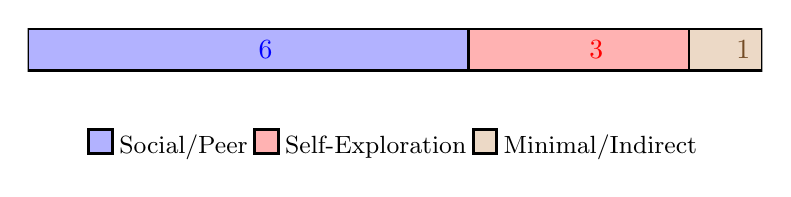
\begin{tikzpicture}
        \begin{axis}[
            xbar stacked,                     % Create a horizontal stacked bar chart
            xmin=0, xmax=10,                  % Set x-axis range (total participants = 10)
            width=0.9\linewidth,              % Chart width relative to text width
            height=3cm,                       % Chart height
            bar width=15pt,                   % Width of the bar segments
            enlarge y limits=0.5,             % Add vertical space around the bar
            axis x line=none,                 % Remove x-axis line
            axis y line=none,                 % Remove y-axis
            xtick=\empty,                     % Remove tick marks
            nodes near coords,                % Display numbers on the bar segments
            nodes near coords align={horizontal},
            nodes near coords style={font=\color{white}},
            legend style={
              at={(0.5,-0.15)},
              anchor=north,
              legend columns=3,
              draw=none,
              font=\small,
              nodes={anchor=base}
          },
          legend image code/.code={
              \draw[fill=#1, draw=black] (0cm,0cm) rectangle (0.3cm,0.3cm);
          },
        ]
            % Add each segment of the stacked bar:
            \addplot+[draw=black, line width=1pt] coordinates {(6,0)};    % Social/Peer Learning (3 participants)
            \addplot+[draw=black, line width=1pt] coordinates {(3,0)};         % Self-Exploration (5 participants)
            \addplot+[draw=black, line width=1pt] coordinates {(1,0)};        % Minimal/Indirect Exposure (2 participants)
            \legend{Social/Peer, Self-Exploration, Minimal/Indirect}
        \end{axis}
    \end{tikzpicture}

\end{document}
